
\chapter{システムの性能評価}\label{chap3}
\section{はじめに}
本章では2章で示したシステムの機器・プロトコルについて,実環境での使用を目標とした性能評価を行った.
また,測定に伴い発生する欠測値の補間方法ならびにノイズの除去方法についても考察・実証のうえまとめた.

\section{TWELITE無線タグの性能評価}\label{TWELITEs}
ここでは,システムのうち,TWELITE無線タグについて,実際の通信距離と電波強度の関係についてまとめた.

\subsection{通信距離と電波強度の関係の定量的な測定}
\subsubsection{測定の条件}
本測定ではMONOSTICKをPCに接続し,MONOSTICKとTWELITE CUEを使用して行った.
周囲に何もない屋内環境(体育館)において,MONOSTICKとTWELITE CUEの距離を1m,2m,3m,4m,5m,10m,15m,20m,25mに固定し30秒間測定した.
測定は2つのTWELITE CUEタグを使用して行い,発信頻度は1.56Hz(加速度サンプリング頻度25Hz,送信サンプル数16)とした.
測定時間30秒間に送られてくる電波強度(LQ値)を平均し,測定結果とした.


\subsubsection{測定結果}
通信距離と電波強度の測定結果は図\ref{LQ25}のようになった.
電波強度は通信距離5mまでは一次関数的な減少を見せたが,その後は多少の上下こそあるもののほぼ横ばいの推移を見せた.


\begin{figure}[!htb]
  \centering
  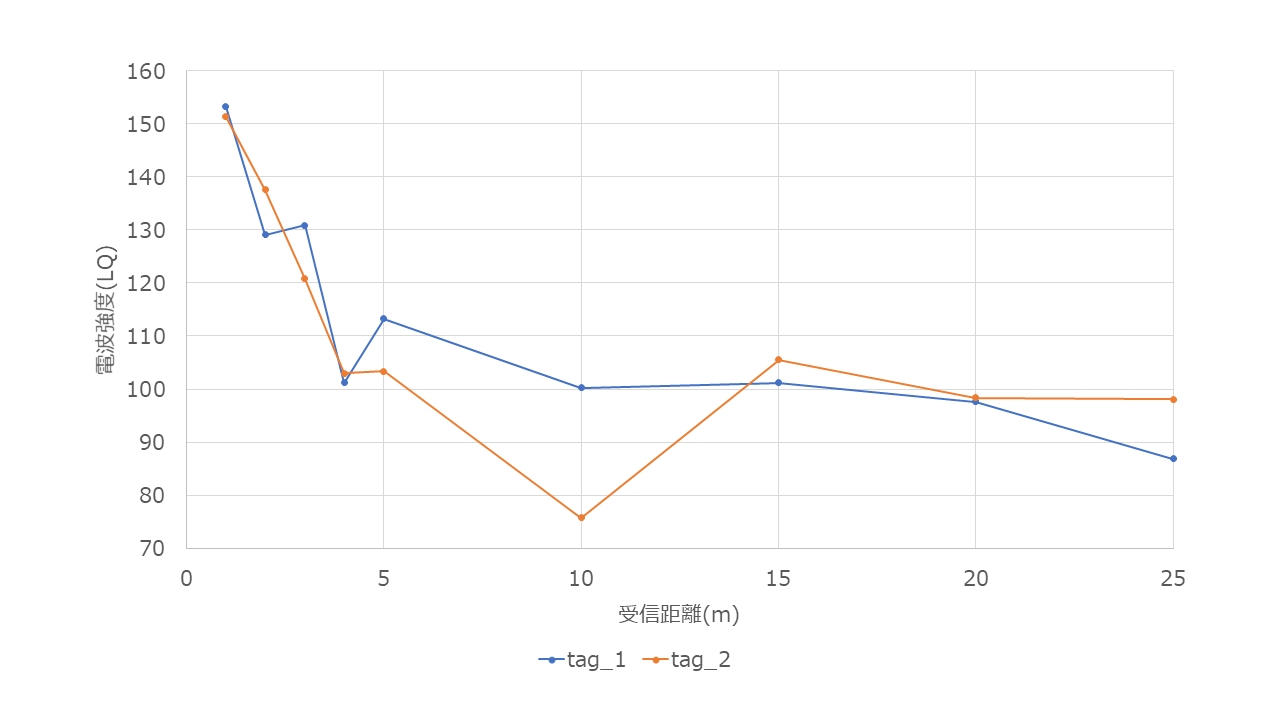
\includegraphics[width = 15cm, bb= 0 0 1000 600]{chapter3/LQ25.png}
  \caption{通信距離と電波強度の測定結果}
  \label{LQ25}
\end{figure}
\clearpage


\subsubsection{測定結果からの考察}
以上の結果より,特異的な結果は通信距離おおむね5m以内で現れるLQ値120以上という値であることが分かった.
よって,以降の研究では通信距離が5m以内となる計測条件を設定して実験を行うこととする.


\subsection{機器の評価を踏まえたTWELITE無線システムの利用方法}
以上の評価結果を踏まえ考えられるTWELITE無線システムの利用方法は以下の通りである.
図\ref{LQ25}からわかるように,TWELITE無線の電波強度は,通信距離5m程度までは単調に減少し,それ以降は横ばいの推移をとる.
このことを用いて,MONOSTICKとTWELITE CUEが5m以下の距離にあるような使い方をする.

\subsubsection{網羅的配置}
まず,MONOSTICKを取り付けたマイコンの配置について,一つのMONOSTICKが受け持つ範囲は,
半径5m以下の円形の範囲とする.
そのうえで,図\ref{sysmodel}のようにカバーしたい範囲を網羅するように配置することで,
子供がいずれかのMONOSTICKと5m以内に近接していることになるので,高い電波強度を示すMONOSTICKが必ず現れる.
それにより子供の位置を概ね特定することができる.
この方法では,値による閾値を示さずとも他との比較により位置を推定できるので簡単である.
\clearpage

\begin{figure}[!tb]
  \centering
  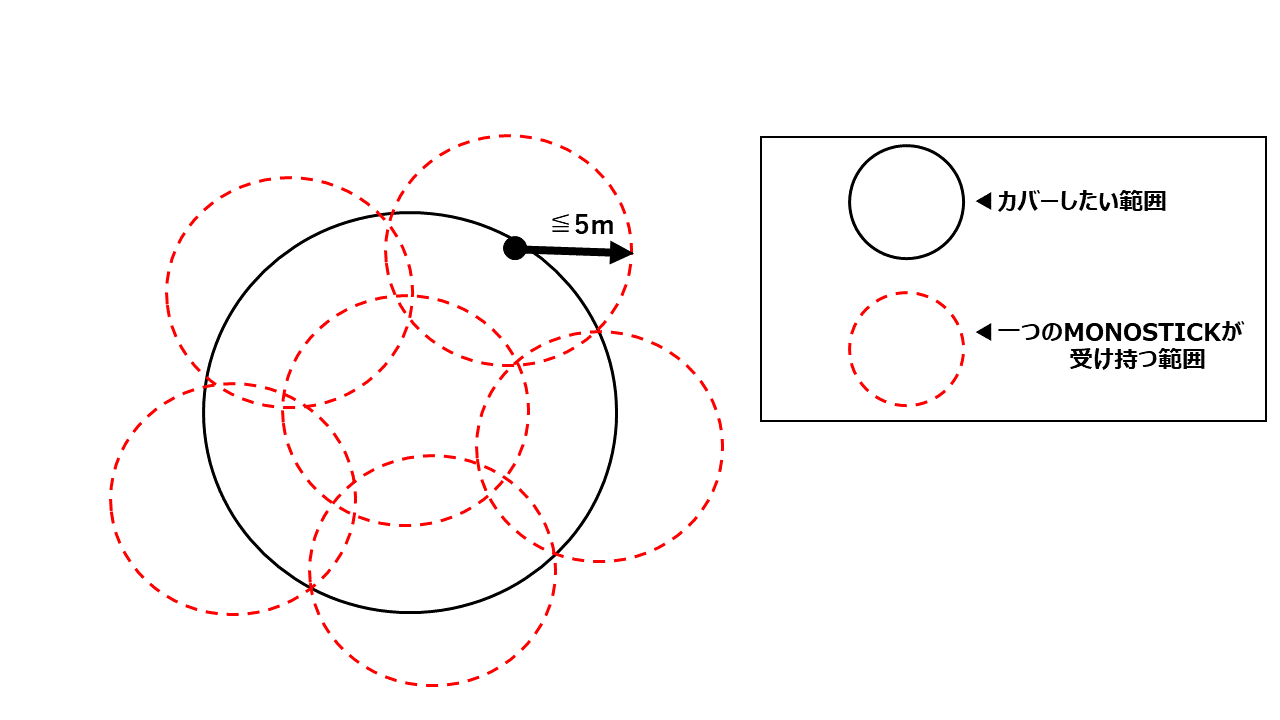
\includegraphics[width = 16cm, bb= 0 0 1000 700]{chapter3/sysmodel.png}
  \caption{MONOSTICKの網羅的配置}
  \label{sysmodel}
\end{figure}



\subsubsection{チェックポイント的配置}
MONOSTICKが受け持つ範囲は同様に半径5m以下とする.
ここで,MONOSTICKが受け持つ範囲の中に,特定の入口・出口ゲートや,滑り台の降り口など,
特定の遊びをしたときに通るポイントを含めることにより,子供が何をしていたかを概ねつかむことができる.
使用するMONOSTICK,マイコンの量を減らせるので,リソースに限りがあるときに有用である.

\clearpage


\section{MQTTプロトコルの性能評価}
つづいて,MONOSTICKを取り付けた複数のマイコンからデータを集約するためのMQTTプロトコルについて評価を行う.
MQTTプロトコルは軽量かつ即時性に優れたプロトコルであるが,実際の使用環境におけるデータの送受信に耐えるか確かめるべく
データ受信のレイテンシや送受信の成功率についてまとめた.

\subsection{測定環境}
MQTTのパブリッシャとしてはMONOSTICKを取り付けたマイコン(Raspberry Pi)を使用し,
ブローカーおよびサブスクライバPCとしてWindows PC1台を使用した.
なお,MQTTはポート1883を使用したTCP/IP通信によって行われる.
LANによる接続はすべてWi-Fiを用いた無線通信により行うこととし,それを実現するためのWi-Fiルーター1台も用いた.
Wi-Fiは屋外利用が想定されることおよび安定した通信を目指すことから2.4GHz帯を使用した.
実際に使用したMQTTの構成詳細を図\ref{MQTTprop}に示した.

なお,本測定で使用したタグからのデータ取得及びMQTTデータ転送のプログラムについて,ソースコードは最後に付録としてまとめてある.

\clearpage

\begin{figure}[htb]
  \centering
   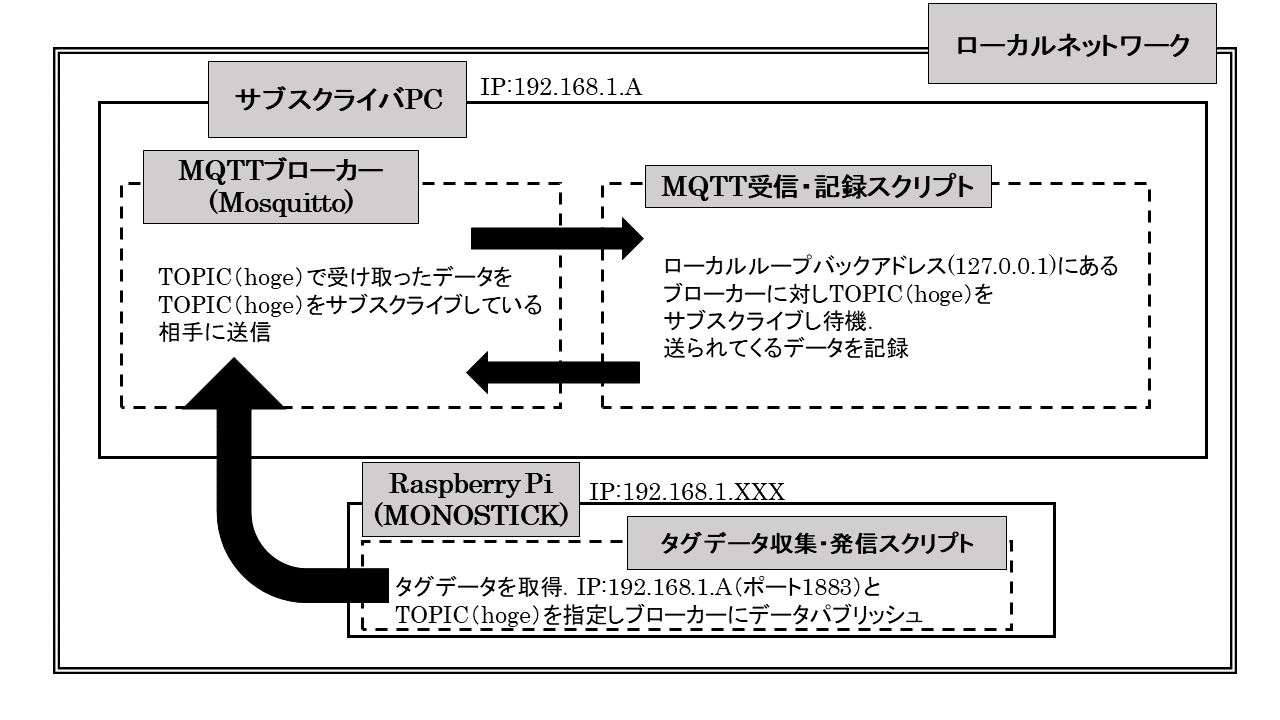
\includegraphics[width = 15.8cm, bb= 0 0 1000 600]{chapter3/MQTTprop.png}
   \caption{MQTTによるやり取りの詳細}
   \label{MQTTprop}
\end{figure}


\subsection{MQTTの受信成功率測定}
受信成功率の測定はMONOSTICKから取得したTWELITE CUEタグからの受信データ(34 Byte)をMQTTプロトコルによって送信する際,パブリッシャ側のマイコンでも同時にログをとることにより行った.
MQTTを介してサブスクライバ側が受け取ったデータとパブリッシャ側に残るデータを照らし合わせ,
データの欠測のうちMQTTプロトコルに起因する欠測の数を計測し受信成功率を求めた.
試行回数6879回のうちMQTTプロトコルに起因するデータの欠測は0件だったため,MQTTの受信成功率は100\%であることが確かめられた.
\clearpage

\subsubsection{時刻の同期に関する問題のMQTTによる解決}
本研究では,複数のマイコンを用いてデータの取得を行うが,複数のマイコンの時刻がずれていると
マイコンごとにTWELITE CUEからのデータ受信時刻が異なることになり,正確な受信時刻を得ることができない.
それを防ぐためには,マイコンの時間を同期する必要があった.
しかし,MQTTが即時性に優れたプロトコルであることを利用して受信時刻をサブスクライバ側のPCの時刻に一括することができれば,
マイコンの時間を同期する必要がなくなる.
本稿ではそのための条件を設定して実験を行った.

\subsection{MQTTのレイテンシ測定}
本研究で送信されているデータの送信頻度は1.5Hz程度である.
よって,レイテンシを0.5秒以内に抑えることができれば前後のデータが入れ替わることなくマイコンの時刻同期をせずとも受信時間に正確さが出る.
本稿では,様々な条件のもとでMQTTプロトコルのレイテンシを測定し,実際に0.5秒以内に抑えられているか確かめた.

\subsubsection{単一パブリッシャからの受信で測定したレイテンシ}
受信成功率と同様にしてMQTTのレイテンシ測定を行った.
レイテンシ測定はパブリッシャのマイコンとサブスクライバのPC双方にMONOSTICKを取り付けることによって行った.
TWELITE CUEから発信されたデータは,パブリッシャのマイコンに取り付けられたMONOSTICKおよびMQTTを介してサブスクライバのPCに届く.
サブスクライバPCでは,MQTTを介してデータが届いた時刻を記録した.
一方,サブスクライバのPCでも同じデータをMONOSTICKのみを介して取得し,その時間も記録した.
その二つの受信時間を比較すればMQTTの遅延時間を求めることができる.
レイテンシの計測結果は以下の表\ref{mqttlate}のようになった.
最大値こそ4秒台と大きいものの,平均,標準偏差ともに小さく抑えられていることからわかる通り,ほとんどの場合では非常に小さい値になっていることが特徴である.

\clearpage

\begin{table}[htb]
 \centering
  \caption{単一パブリッシャからの受信で測定したレイテンシ}
  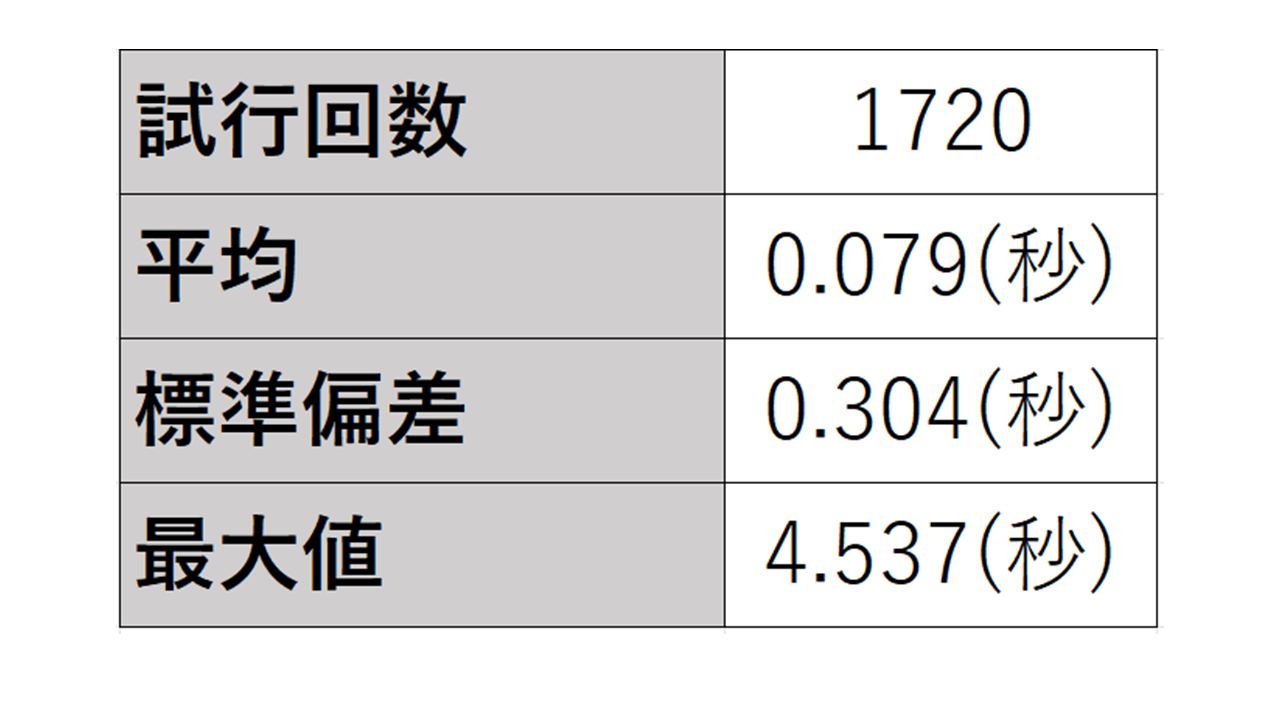
\includegraphics[width=7cm, bb= 0 0 1200 600]{chapter3/mqttlate.png}
  \label{mqttlate}
\end{table}

\subsubsection{複数パブリッシャからの受信で最速をとったレイテンシ}
本研究で想定されているシステムではTWELITE CUEからのデータは複数のマイコン・MQTTパブリッシャを通して届く.
そのため,複数のパブリッシャから送られた同一時刻の情報のうち,一番最初にサブスクライバに届いた時刻を代表として記録すればレイテンシを抑えることができる.
4台のマイコンを用意し,それぞれにMONOSTICKを取り付け,同一のサブスクライバに向けてMQTTで情報を送信した.
単一パブリッシャでの実験と同様に,MQTTを通してサブスクライバに届いた時刻を記録し,同一データに関する時刻のうち一番早いものを比較のための代表時刻とした.
サブスクライバのPCにもMONOSTICKを取り付けTWELITE CUEからのデータを記録し,受信時間を比較しレイテンシとした.
レイテンシの計測結果は以下の表\ref{mqttlate2}のようになった.
最大レイテンシは0.5秒以下に抑えられているため,本研究ではマイコンの時刻の同期は行わず,記録する時刻はMQTT受信後のサブスクライバの時刻とする.

\begin{table}[htb]
  \centering
   \caption{複数パブリッシャからの受信で測定したレイテンシ}
   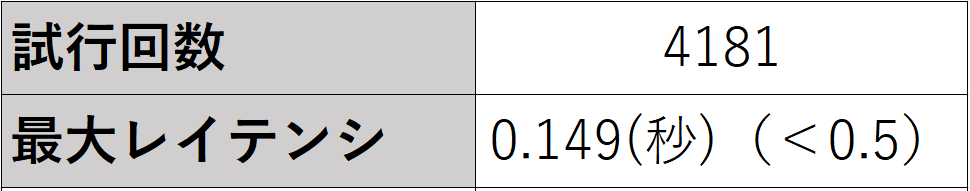
\includegraphics[width=7cm, bb= 0 0 800 250]{chapter3/mqttlate2.png}
   \label{mqttlate2}
\end{table}

\clearpage

\section{データの処理方法の決定}
ここでは,TWELITEタグ及びMQTTプロトコルを用いて集約されたデータに発生するノイズの除去や欠測値の補間について述べる.

\subsection{状態空間モデルを用いたフィルタの適用}
一般に,あるシステムを運用する際に,実際にはシステムの状態を直接確認できず,環境や観測機器によるシステムノイズや観測ノイズが生じる.
このノイズはある分散をもった正規分布に従うと仮定してフィルタリングすることができ,計量や信号処理などの分野で活用されている.
本研究で得られる測定結果も,電波干渉等に影響され得られるデータには振動が生じているため,状態空間モデルを用いたフィルタを使用しノイズを除去する.
フィルタリングは以下の式\ref{kal1},\ref{kal2}に基づいて行われる.
\begin{equation}
 \label{kal1}
 x_n = Fx_{n-1} + Gv_n 
\end{equation}

\begin{equation}
  \label{kal2}
  y_n = Hx_n + w_n
\end{equation}

ここで,
\it
F,G,H
\rm
は適切な次元を持つ行列で,
\it
$v_n$,$w_n$
\rm
は平均0でそれぞれ$\tau^2$,$\sigma^2$
を分散とする正規分布に従うとする.\cite{TSSS}
状態空間モデルでは,時間更新(Predict)により$x$の一歩先の状態を予測し,実際の観測値$y$によって推定値の更新(Correct)を行う.\cite{kalman}
本稿では,これを利用し,適切な$\tau^2$の値を用いることで$x$の状態を推定する.
図\ref{kalman}は測定されたデータセットに対し$\tau^2 = 0.1$としてフィルタリングした結果である.
得られた測定値の特徴を残しつつノイズの除去が行われている.

\clearpage
\begin{figure}[!t]
  \centering
  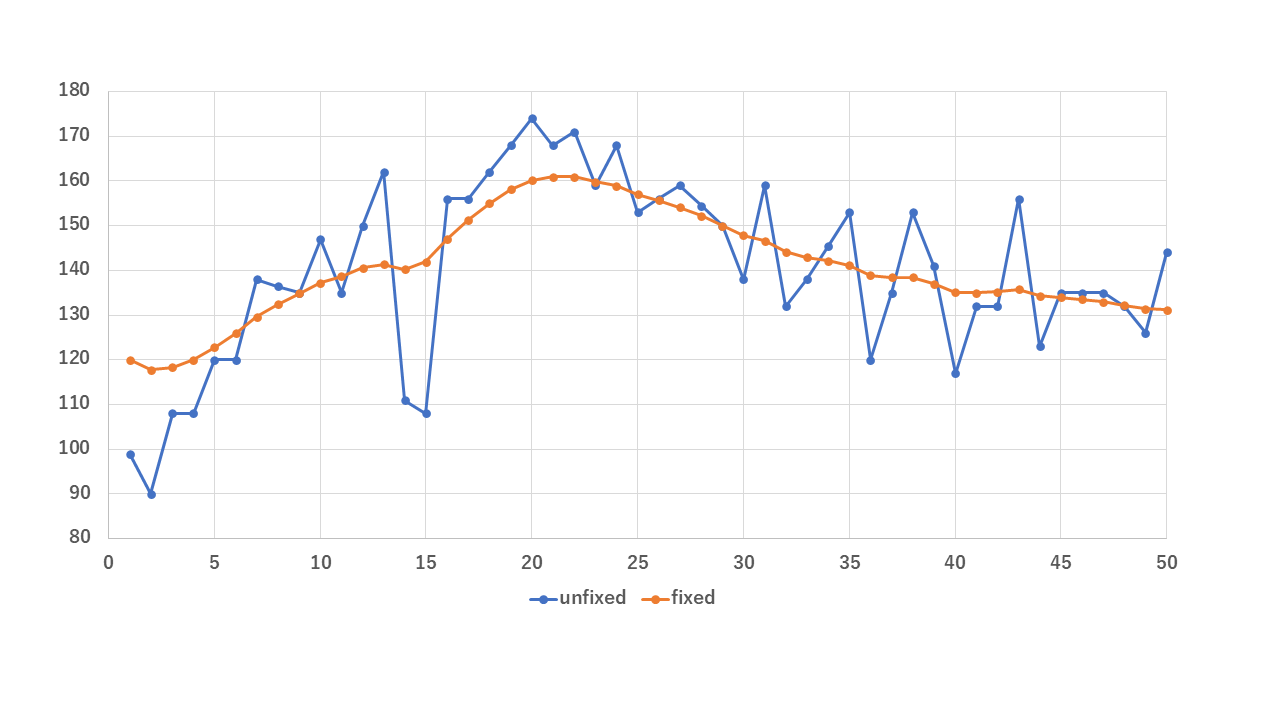
\includegraphics[width = 15cm, bb= 0 0 1000 500]{chapter3/kalman.png}
  \caption{状態空間モデルを用いたフィルタリング結果}
  \label{kalman}
\end{figure}



\subsection{欠測値の補間方法}
前述した状態空間フィルタを適用するためにはデータを時系列データとする必要がある.
しかし,TWELITE CUE・MONOSTICKを用いた実験では,データの発信頻度にかかわらずデータの欠測が生じる.
複数のMONOSTICKを使用して同一のデータを複数経路で受信している場合,
受信しているうちの一部が欠測により不足していることがある.
この場合,正しい比較ができなくなるため適切な方法で欠測を補間する必要がある.
ここでは,適切に補間するための方法について検討する.

\subsubsection{NN補間}
NN(Nearest\ Nearby)補間は,一番単純な補間方法で,欠測が発生した部分の前後
のデータのうち,該当部に近いほうのデータを用いてそのまま補間する.

\subsubsection{線形補間}
線形(linear)補間は,欠測が発生した部分の前後のデータ間で,値が線形な変化をしたと仮定し,その値で補間する方法である.

\subsubsection{スプライン補間}
(三次)スプライン(spline)補間は,N個の測定点(データ)が与えられたデータセットをN-1個の区間に分割し,その区間ごとに適切な三次曲線を求めてそれをもとに補間する方法である.
区間ごとの三次曲線は以下の条件を満たす.
\begin{quote}
  \begin{itemize}
   \item 各区間を補間する曲線はその両側の点を通る.
   \item N個の各点において両側の区間の1次導関数は等しい.
   \item N個の各点において両側の区間の2次導関数は等しい.
  \end{itemize}
\end{quote}
三次曲線の未知数4つに対して,式が4つできるのでこの条件により各区間ごとに補間する曲線の式が求まることを利用し補間するのがスプライン補間である.

\subsection{補間方法の比較}
先に述べた三つの補間方法の比較のため,実際に計測できたデータセットからランダムに一部を削除し,
欠測のある状態を作り出した.そのうえで実際の計測データ(unfixed)とそれぞれの補間方法で補間されるデータを示したのが図\ref{interp}である.
まず,スプライン補間は,各測定点の両側で1次導関数,2次導関数が等しいという条件に影響され,データの上下が激しい区間で欠測した場合に
オーバーシュートが発生するため,補間方法として適切ではないことが分かった.
よって,線形補間とNN補間に絞って比較した.
この二つの補間方法による差は大きくないが,実際の子供の移動により近いと考えられるのは線形補間であるため,本稿では線形補間により補間を行うこととする.

\begin{figure}[!htb]
  \centering
  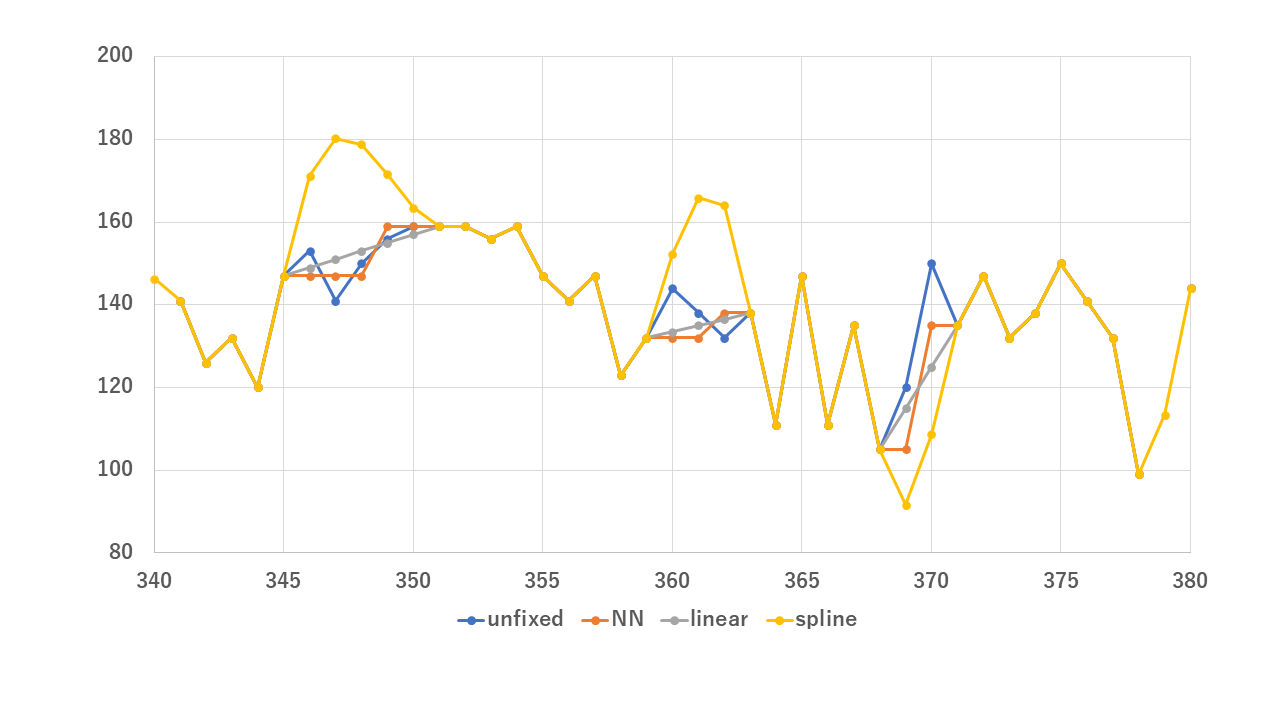
\includegraphics[width = 15cm, bb= 0 0 1000 600]{chapter3/interp.png}
  \caption{補間方法の比較}
  \label{interp}
\end{figure}


